%%%%%%%%%%%%
%% Please rename this main.tex file and the output PDF to
%% [lastname_firstname_graduationyear]
%% before submission.
%%%%%%%%%%%%

\documentclass[12pt]{caltech_thesis_progress2}
\usepackage[hyphens]{url}
\usepackage{lipsum}
\usepackage{graphicx}
\usepackage{svg}
\usepackage{todonotes}
\usepackage{hyperref}
\usepackage{dirtytalk}
\usepackage{float}
\hypersetup{
    colorlinks,
    linkcolor={red!50!black},
    citecolor={blue!50!black},
    urlcolor={blue!80!black}
}
\renewcommand{\chaptername}{}
\AtBeginDocument{\renewcommand{\bibname}{References}}
%% Tentative: newtx for better-looking Times
\usepackage[utf8]{inputenc}
\usepackage[T1]{fontenc}
\usepackage{newtxtext,newtxmath}
\usepackage[backend=bibtex,
style=numeric,
bibencoding=ascii,
sorting=none
%style=alphabetic
%style=reading
]{biblatex}

%\renewcommand{\familydefault}{\rmdefault}
% Must use biblatex to produce the Published Contents and Contributions, per-chapter bibliography (if desired), etc.
% Name of your .bib file(s)
\addbibresource{example.bib}
\addbibresource{ownpubs.bib}

\begin{document}

% Do remember to remove the square bracket!
\title{Information-Performance Tradeoffs in Control}
\author{Ayush Pandey}

%\degreeaward{Visiting Undergraduate Research Program}                 % Degree to be awarded
\university{California Institute of Technology}    % Institution name
\address{Pasadena, California}                     % Institution address
\unilogo{caltech.png}                                 % Institution logo
\copyyear{July 2016}  % Year (of graduation) on diploma
\defenddate{17th June}          % Date of defense
%
%\orcid{[Author ORCID]}

%% IMPORTANT: Select ONE of the rights statement below.
%\rightsstatement{All rights reserved\todo[size=\footnotesize]{Choose one from the choices in the source code!! And delete this \texttt{todo} when you're done that. :-)}}
% \rightsstatement{All rights reserved except where otherwise noted}
% \rightsstatement{Some rights reserved. This thesis is distributed under a [name license, e.g., ``Creative Commons Attribution-NonCommercial-ShareAlike License'']}

%%  If you'd like to remove the Caltech logo from your title page, simply remove the "[logo]" text from the maketitle command
\maketitle[logo]
%\maketitle

%\begin{acknowledgements} 	 
%   [Add acknowledgements here. If you do not wish to add any to your thesis, you may simply add a blank titled Acknowledgements page.]
%\end{acknowledgements}
%
%\begin{abstract}
%   [This abstract must provide a succinct and informative condensation of your work. Candidates are welcome to prepare a lengthier abstract for inclusion in the dissertation, and provide a shorter one in the CaltechTHESIS record.]
%\end{abstract}

%% Uncomment the `iknowhattodo' option to dismiss the instruction in the PDF.
%\begin{publishedcontent}%[iknowwhattodo]
%% List your publications and contributions here.
%\nocite{Cahn:etal:2015}
%\end{publishedcontent}

\tableofcontents
%\listoffigures
%\listoftables
%\printnomenclature

\mainmatter
\chapter{Introduction}
We deal with two important settings of networked control systems where information theory bottlenecks need to be considered viz. the rate limited communication of data between observer and controller and communication over AWGN (Additive White Gaussian Noise) channel. We will briefly present the existing results with respect to the two settings. The problems being considered in this project would be forumalated next. The reader is referred to the previous documents, the progress report and the project proposal on this project for various preliminaries and previous results in this project. 
	\section{Motivation}
It is often the case that the observer and the controller are not physically connected together in a networked control system. Hence, in any implementation of such a control system, having a rate limited channel is inevitable. Moreover, it is common that this communication channel would be corrupted with noise. Hence, it is of paramount importance to deal with such control systems because a finite rate of communication and addition of noise leads to degradation in performance of the system. In this project, we aim to study the tradeoff between performance of the system and effect of noisy or rate limited communication channel. 
\section{Background}
In the past decade, the problems regarding control with communication constraints have been considered in detail. Recently, in \cite{anatoly} a slightly different scheme was proposed for multi-rate control over AWGN channel. \cite{victoria} gives lower and upper bounds to the LQG performance cost when the system is under limited rate of communication constraint. 
The reader is referred to citations in \cite{anatoly} and \cite{victoria} for a detailed literature review of these topics. 
\chapter{Objectives}
We broadly divide the work into two parts as mentioned in the Introduction. We would be dealing with the problem of AWGN communication channel similar to \cite{anatoly}. In \cite{anatoly}, it has been assumed that the system disturbance $w$ are i.i.d. Gaussian. We study the cases when this system disturbance is not Gaussian but some other random distribution. The problem would be formulated exactly as given in \cite{anatoly}, with the only difference being that we wouldn't assume the system disturbances $w$ to be Gaussian. Next, we would study the bounds on the performance cost for the rate-limited noiseless communication channel. The results for lower and upper bounds have been given \cite{victoria}. We aim to compare the performance of a simple uniform quanitzation scheme with the upper and lower bound results given in \cite{victoria}. For this problem, the system setting would be exactly as given in \cite{victoria}. The general system scheme is presented below.
% along with a diagramatical representation in Fig.(\ref{system_diag}).
%\begin{figure}[H]
%
%			  \centering
%%			  \includesvg[width=1.0\textwidth]{block2}
%%			  \def\svgscale{5.5}
%%			  \tiny{
%%			  \input{ulft.pdf_tex}}
%			\includegraphics[scale=0.5]{system_diag}
%			  \caption{The general control system block diagram in consideration with rate limited communication channel or an AWGN channel between observer and controller}
%			 \label{system_diag}
%		\end{figure}	
	\section{Problem Formulation}
	\label{problem}
		Consider a discrete time system,
			\begin{align}
			\label{system}
				x_{t+1}&=A_{t}x_{t} + u_{t} + w_{t}\\
				y_{t}&=x_{t}+v_{t}
			\end{align}
			where $A_{t}$ is the system parameter, $w_{t}$ and $v_{t}$ are system disturbance and noise in observation respectively, independent of each other. $x_{t}$ are the system states, with known statistical properties of $x_{0}$, which is assumed to be independent of the noises. and $y_{t}$ are the measurements. We only consider a scalar case for now.\\

\chapter{Project Progress}

\section{Control over AWGN Channel}
To study the tradeoff between performance and effect of noise in communication channel when the system has non-Gaussian disturbances, we first find an expression between optimal cost achieved vs SNR of the channel for the Gaussian disturbance case itself. Using \cite{lqg} for the partially observed case and fixing up the variables to match the system setting in \cite{anatoly} we obtained the following expression for optimal cost ($J^{*}$) in terms of SNR for scalar case:
	\begin{align}
	\label{computedJ}
	 J^{*} &= \sum\limits_{t = 0}^{T} \left[Q\Sigma(t) + \left(S(t)\left(A^{2}\Sigma(t-1) + W - \Sigma(t)\right)\right)\right]\\
	 \intertext{where $S(t)$ is obtained using controller ARE (see \cite{anatoly}), $W$ is variance of the system disturbance, $Q$ is the weight in the LQG cost, $\Sigma(t)$ is obtained using Kalman filter gains $P(t)$ as shown in \cite{anatoly} as follows}
	 \Sigma(t) &= \frac{P(t)-W}{A^{2}}\\
	 P(t+1) &= A^{2}P(t)\left(1-\frac{P(t)}{P(t)+V}\frac{SNR}{1+SNR}\right)+W
	\end{align}	 
Simultaneously, we simulated the system as given in Eq.(\ref{system}) following the step by step scheme given in \cite{anatoly}. Simulating for each time instant, we ended up calculating the simulated performance cost. To verify the results obtained, we plotted on the same curve the computed optimal performance cost (from Eq.(\ref{computedJ})) and the simulated optimal performance cost by simualting the system step by step for each time instant. The resulting plot for a fully observable system ($v = 0$) is shown in Fig.(\ref{comp_vs_sim}). 
		\begin{figure}[H]
			 \centering
%			
				\tiny{
%			  \resizebox{5in}{!}{\input{lowerBound_Simulation_rateLimitedLQG.pdf_tex}}
			\includesvg[width=16cm]{computed_vs_simulated_snr30_manyTime}}
%			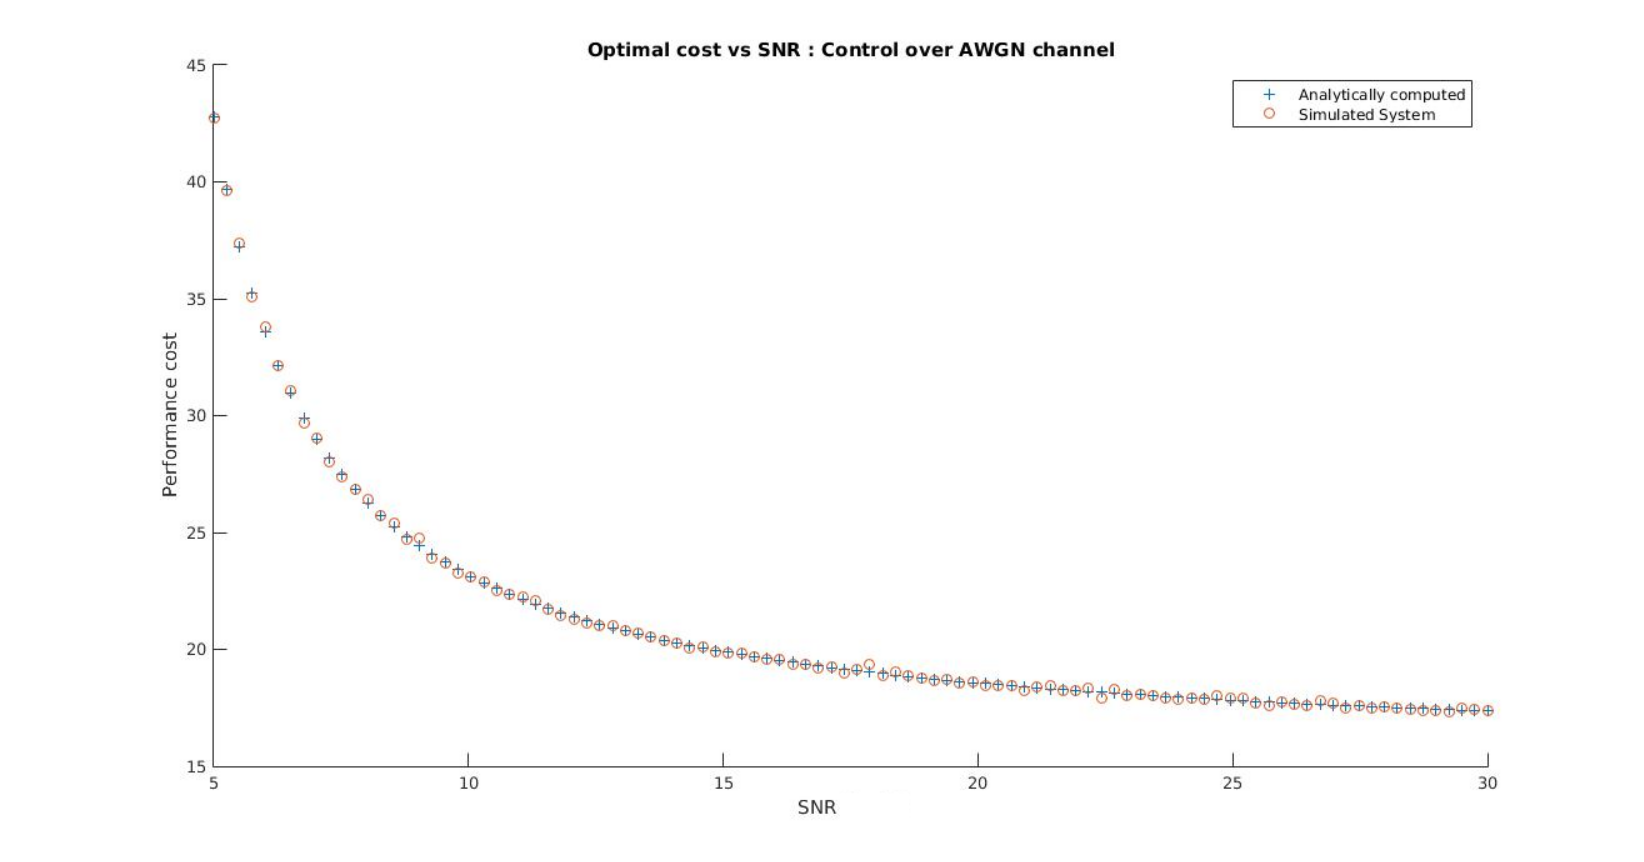
\includegraphics[scale=0.27]{computed_vs_simulated_snr30_manyTime}
					  
			  \caption{Comparing the computed optimal cost with the simulated optimal cost for system with AWGN communication channel. The fully observable system has the parameter $A = 2$ and the system disturbance $w$ is zero mean Gaussian with $\sigma_{w} = 1$.}			 
			 \label{comp_vs_sim}
		\end{figure}	
Similarly, for partially observeable case with Gaussian noise $v$ in measurement (i.e. $y = x + v$), we make the appropriate changes and compare the computed and the simulated optimal performance cost vs SNR on the same plot. The resulting plot is shown in Fig.(\ref{comp_vs_sim_v}).
	\begin{figure}[H]
			  \centering
			\tiny{	
%			  \resizebox{5in}{!}{\input{lowerBound_Simulation_rateLimitedLQG.pdf_tex}}
			\includesvg[width=16cm]{control_over_AWGN_withV_GaussianW}}
%			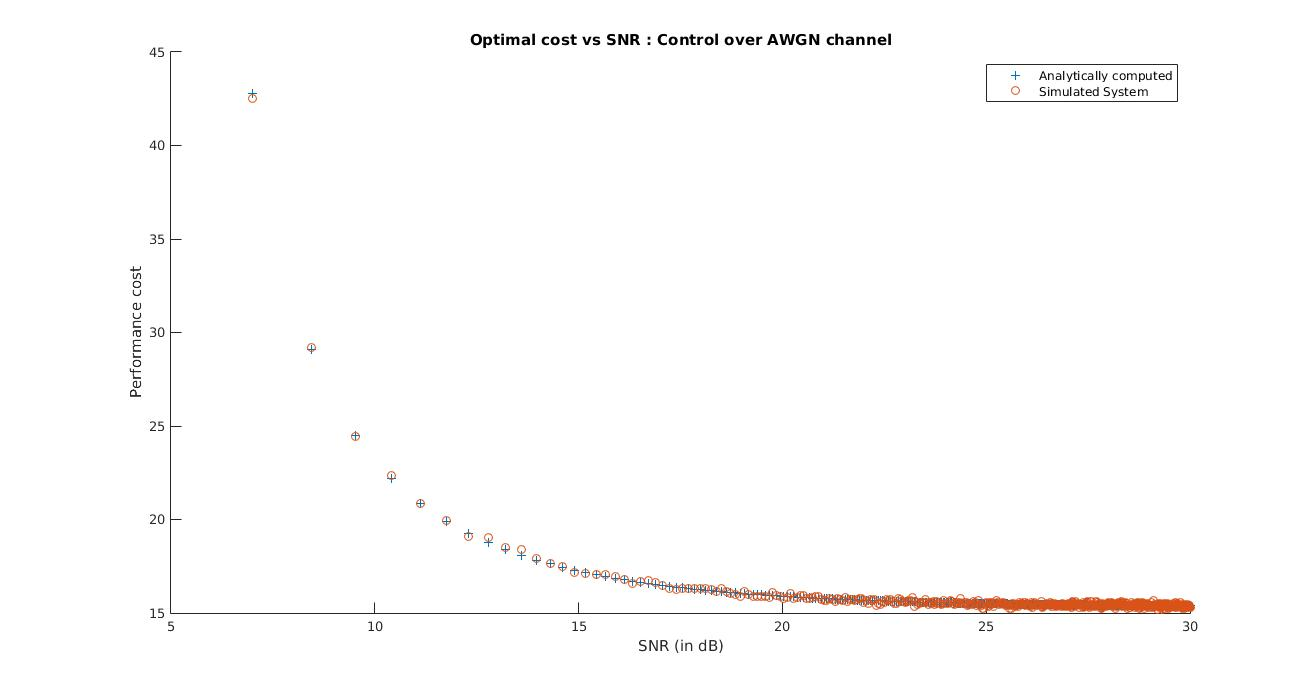
\includegraphics[scale=0.27]{computed_vs_simulated_SNRdB30}
			  \caption{Comparing the computed optimal cost with the simulated optimal cost for system with AWGN communication channel. The partially observable system has the parameter $A = 2$, the system disturbance $w$ is zero mean Gaussian with $\sigma_{w} = 1$ and the noise in measurement $v$ is also zero mean Gaussian with $\sigma_{v} = 1$.}
			 \label{comp_vs_sim_v}
		\end{figure}	
		To tackle the problem of non-Gaussian system disturbance $w$, we use the result derived in \cite{victoria}. The following equation gives the lower bound to the rate distortion function in terms of optimal cost $b$. 
	\begin{equation}
	\mathbb{R}(b) \geq log(|det(A)|) + \frac{n}{2} log \left( 1 + \frac{N(w)|det(M)|^{\frac{1}{n}}}{(b-b_{min})/n}\right)
	\label{lowerbound}
	\end{equation}	
	where $b_{min}$ is the minimum cost as calculated for the classical LQG case and $N(w)$ is the entropy power given by 
	\begin{equation}
	N(w) = \frac{1}{2 \pi e} exp \left( \frac{2}{n} h(w) \right)
	\end{equation}
	where $h(w)$ is the differential entropy of $w$.\\		
	We use the concept of channel capacity to use the above relation for the AWGN channel case in the setting of \cite{anatoly}. The lower bound given in Eq.(\ref{lowerbound}) is valid for any distribution of system disturbance $w$. The channel capacity for noise corrupted channel is given by
	\begin{equation}
		\mathbb{C} = \frac{n}{2} log\left( 1 + SNR \right)
	\end{equation}
	where SNR is the signal to noise ratio of the AWGN channel. We replace the channel capacity in Eq.(\ref{lowerbound}), $\mathbb{R}(D)$, with that given above for the AWGN channel to obtain the expression between optimal cost and SNR for non-Gaussian system disturbance $w$.
	 \\Now, to check the tightness of the lower bound, we simulate the system and compare it with the lower bound plot as shown in Fig.(\ref{lowerbound_vs_laplace}). We used a Laplace distribution for $w$ (with zero mean and $\sigma_{w} = 1$) to simulate and to calculate the lower bound. 
		\begin{figure}[H]
			  \centering
			 \tiny{	
%			  \resizebox{5in}{!}{\input{lowerBound_Simulation_rateLimitedLQG.pdf_tex}}
			\includesvg[width=16cm]{laplaceW_bound_simulation_withoutV}}
%			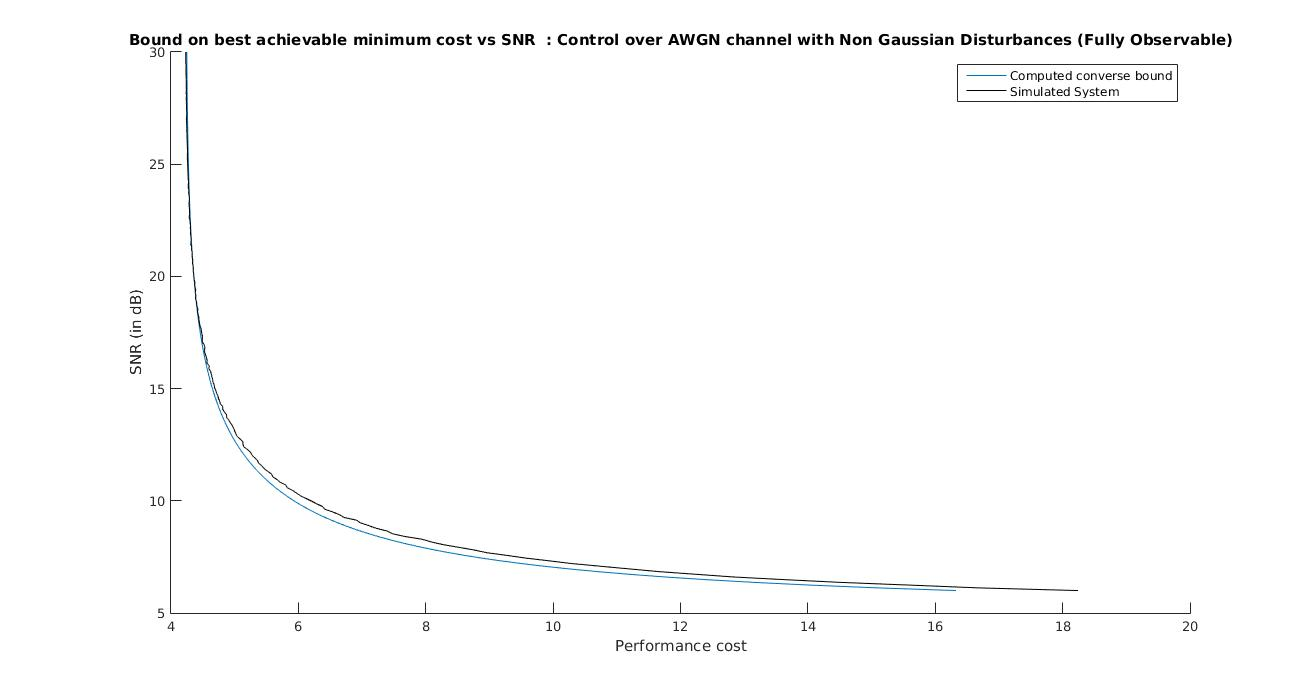
\includegraphics[scale=0.27]{laplaceW_bound_simulation_withoutV}
			  \caption{Comparing the computed optimal cost with the simulated optimal cost for system with AWGN communication channel. The fully observable system has the parameter $A = 2$ and the system disturbance $w$ is zero mean Laplacian with $\sigma_{w} = 1$.}
			 \label{lowerbound_vs_laplace}
		\end{figure}	
		 Similarly, for the partially observable case (i.e. $y = x + v$), we have the modified lower bound from \cite{victoria} given in Eq.(\ref{lowerbound_v})
			  \begin{equation}
			  \mathbb{R}(b) \geq log(|det(A)|) + \frac{n}{2} log \left( 1 + \frac{\left(|det(C(T-\Sigma_{W})C^{T} + \Sigma_{V})|^{\frac{1}{n}} + |detC^{T}C|^{\frac{1}{n}}N(w)\right)|det KM|^{\frac{1}{n}}}{(b-b_{min})/n}\right)
			  \label{lowerbound_v}
			  \end{equation}
			  where $C=1$ and $T,\Sigma_{V}, \Sigma_{W}, K, M$ are obtained by solving AREs for classical LQG control. For details see \cite{victoria}.\\
			  Using the channel capacity concept as for the fully observable case, we convert the lower bound in Eq.(\ref{lowerbound_v}) to get an expression for cost with the SNR of the AWGN channel for the partially observable case. The plot comparing the simulation and computed lower bound for partially observable case is given in Fig.(\ref{lowerbound_vs_laplace_v})
			  \begin{figure}[H]
			  \centering
			 \tiny{	
%			  \resizebox{5in}{!}{\input{lowerBound_Simulation_rateLimitedLQG.pdf_tex}}
			\includesvg[width=16cm]{laplaceW_bound_simulation_withV}}
%			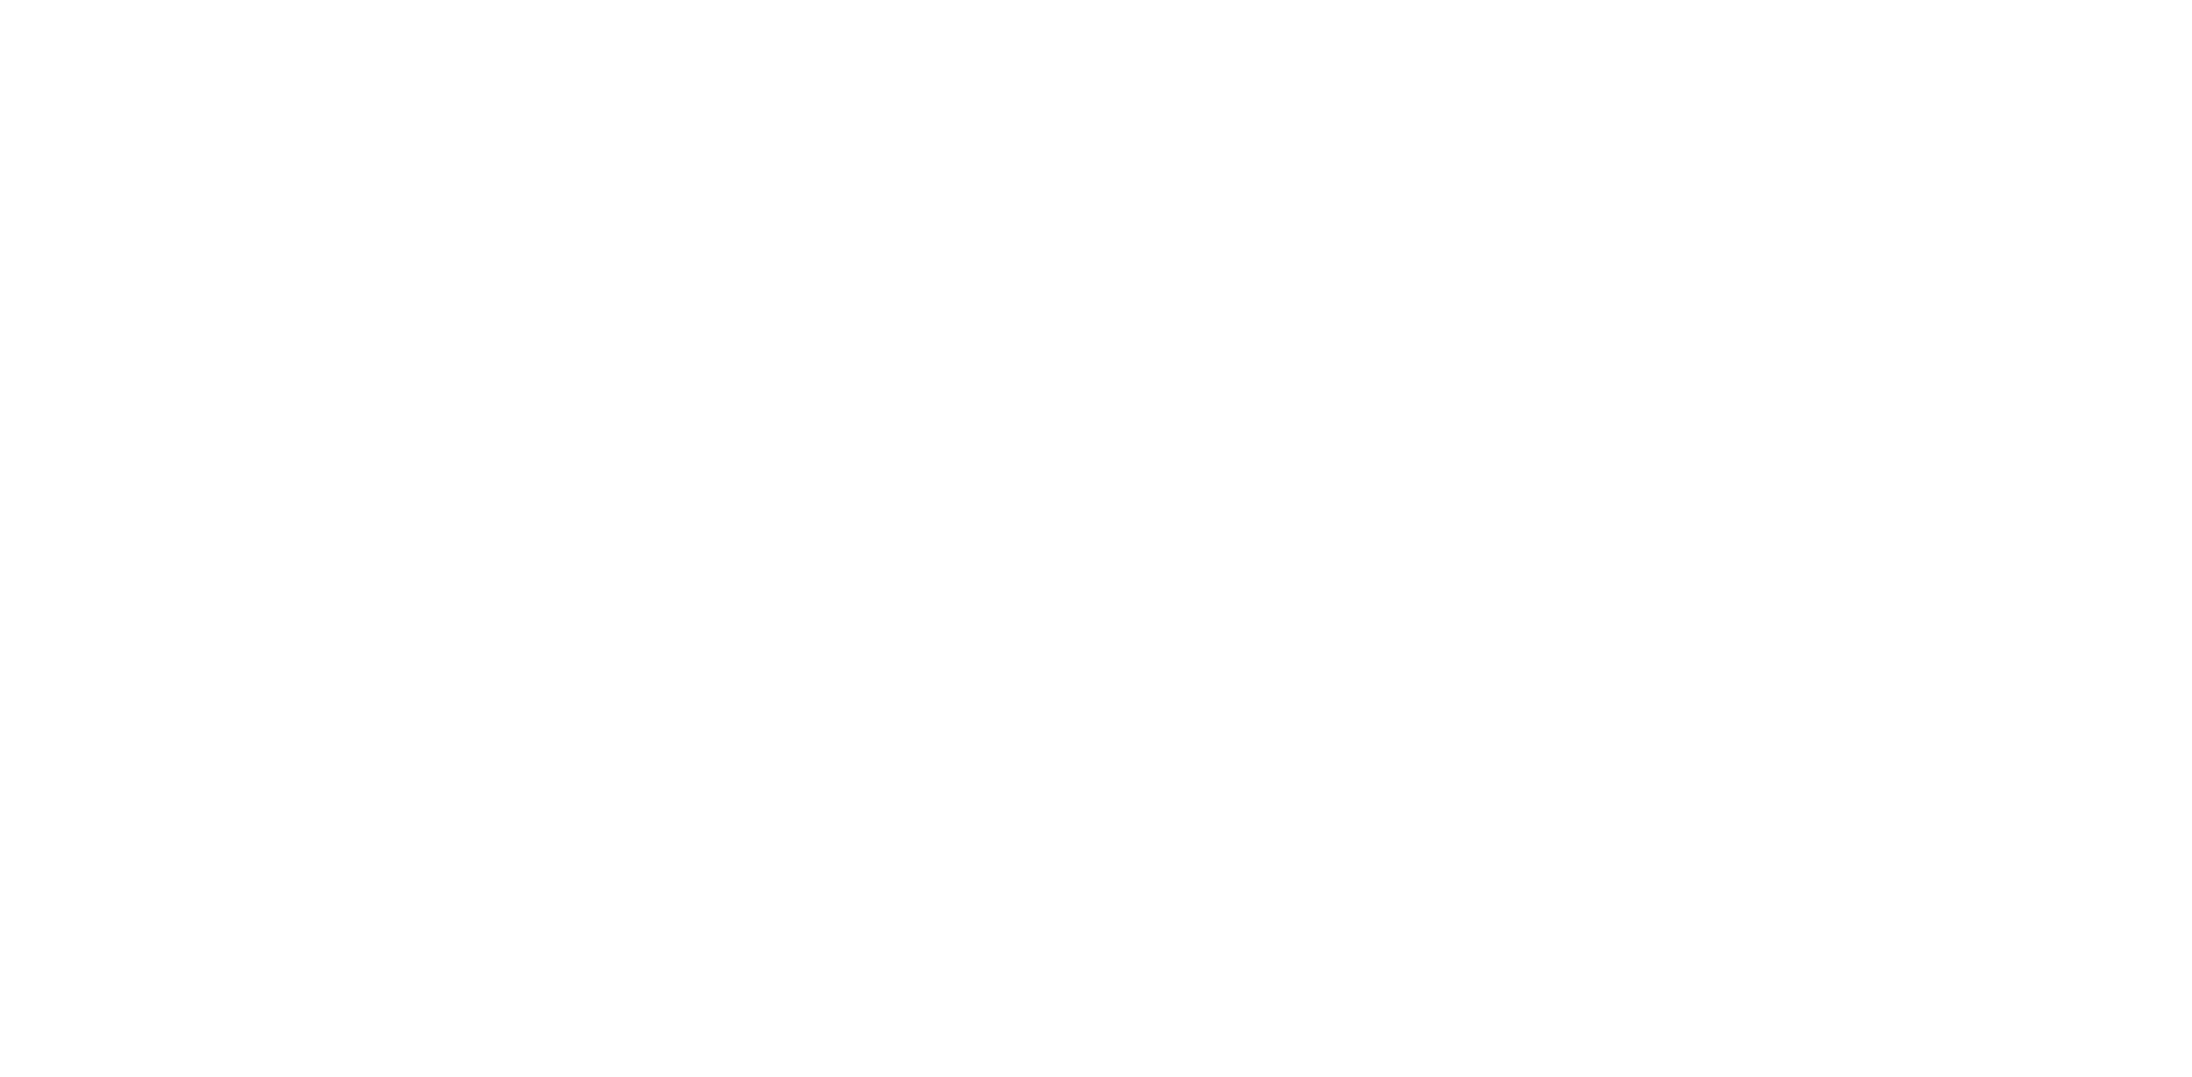
\includegraphics[scale=0.27]{laplaceW_bound_simulation_withV}
			  \caption{Comparing the computed optimal cost with the simulated optimal cost for system with AWGN communication channel. The partially observable system has the parameter $A = 2$, the system disturbance $w$ is zero mean Laplacian with $\sigma_{w} = 1$ and observation noise is assumed to be zero mean Gaussian with $\sigma_{v} = 1$}
			 \label{lowerbound_vs_laplace_v}
		\end{figure}	
	\section{Rate Limited Channel}
		For the case where channel is noiseless but with limited rate of communication, we use the bounds as given in Eq.(\ref{lowerbound}) and Eq.(\ref{lowerbound_v}) for the fully observable and partially observable case respectively.  To simulate the system we use the simplest of the scheme, i.e. a uniform quantizer. The rate distortion function given in Eq.(\ref{lowerbound}) and Eq.(\ref{lowerbound_v}) is upper bounded by the output of the quantizer entropy. Hence, we use the entropy of the quantizer to compute the performance cost lower and upper bounds. Also, we simulate the simple uniform quantization scheme along with the bounds to study the tightness of the bounds obtained in \cite{victoria}.
		\\To calculate the output entropy of the quantizer in the simulated system, we estimate the probabilities of each sample falling in the different quantization bins. Then we use $H(x) = \sum\limits_{i} P_{i}(x)log\left(\frac{1}{P_{i}(x)}\right)$, to calculate the entropy of the quantizer output for each $\Delta$ (the quantizer step size), the quantizer step size. 
		The Fig.(\ref{lowerboundQ_sim}) shows the lower bound to the cost vs quantizer entropy compared with the simulation of the system which is fully observable. 
		\begin{figure}[H]
			  \centering
%			  \includesvg[width=1.0\textwidth]{block2}
%			  \def\svgscale{5.5}
			  \tiny{
%			  \resizebox{5in}{!}{\input{lowerBound_Simulation_rateLimitedLQG.pdf_tex}}
			\includesvg[width=16cm]{lowerBound_Simulation_rateLimitedLQG}}
			  \caption{Comparing the lower bound to the computed optimal cost with the simulated optimal cost for system with rate limited channel. The fully observable system has the parameter $A = 2$, and the system disturbance $w$ is zero mean Gaussian with $\sigma_{w} = 1$}
			 \label{lowerboundQ_sim}
		\end{figure}	
		Similarly, for partially observable case, the plot is drawn and is shown in Fig.(\ref{lowerboundQ_sim_v}).
		\begin{figure}[H]
			  \centering
%			  \includesvg[width=1.0\textwidth]{block2}
%			  \def\svgscale{5.5}
			  \tiny{
%			  \input{ulft.pdf_tex}}
			\includesvg[width=16cm]{lowerBound_Simulation_GaussianDist_rateLimited_partiallyObservedLQG}}
			  \caption{Comparing the lower bound to the computed optimal cost with the simulated optimal cost for system with rate limited channel. The partially observable system has the parameter $A = 2$, the system disturbance $w$ is zero mean Gaussian with $\sigma_{w} = 1$ and observation noise is assumed to be zero mean Gaussian with $\sigma_{v} = 1$}
			 \label{lowerboundQ_sim_v}
		\end{figure}	
In \cite{victoria}, an expression for upper bound to the rate distortion function is also given. This bound is only valid for a fully observable system. Please refer to Theorem 3 in \cite{victoria}.	
	To study the tightness of the upper bound, first we show the plot comparing the lower bound and the upper bound in Fig.(\ref{lower_upper}).
	\begin{figure}[H]

			  \centering
%			  \includesvg[width=1.0\textwidth]{block2}
%			  \def\svgscale{5.5}
			  \tiny{
%			  \input{ulft.pdf_tex}}
			\includesvg[width=16cm]{lowerBound_upperBound}}
%			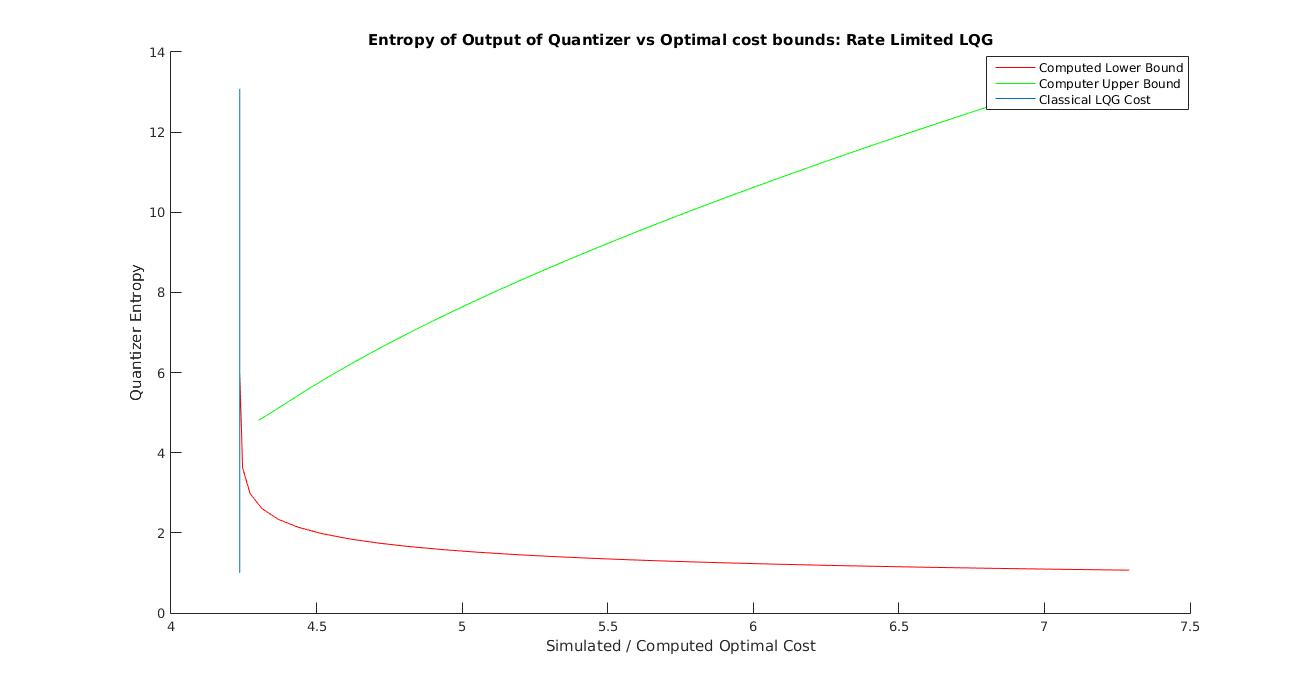
\includegraphics[scale=0.33]{lowerBound_upperBound}
			  \caption{Comparing the lower bound and upper bound to the optimal cost in the rate limited channel case. The fully observable system has the parameter $A = 2$ and the system disturbance $w$ is zero mean Gaussian with $\sigma_{w} = 1$}
			 \label{lower_upper}
		\end{figure}	
		In Fig.(\ref{lower_upper_sim}), the curve for simulation of the system with a uniform quanitzer is also added.
		\begin{figure}[H]
			  \centering
%			  \includesvg[width=1.0\textwidth]{block2}
%			  \def\svgscale{5.5}
			  \tiny{
%			  \input{ulft.pdf_tex}}
			\includesvg[width=16cm]{lowerBound_Simulation_UpperBound}}
			  \caption{Comparing the lower bound and upper bound to the optimal cost in the rate limited channel case with the system simulation for simple uniform quantization scheme. The fully observable system has the parameter $A = 2$ and the system disturbance $w$ is zero mean Gaussian with $\sigma_{w} = 1$}
			 \label{lower_upper_sim}
		\end{figure}	
		
		The plots shown above are not restricted to a particular description of $w$, to demonstrate the fact, the following figures have been given for the case where system disturbance has a Laplace distribution. 
		\begin{figure}[H]

			  \centering
%			  \includesvg[width=1.0\textwidth]{block2}
%			  \def\svgscale{5.5}
			  \tiny{
%			  \input{ulft.pdf_tex}}
			\includesvg[width=16cm]{lowerBound_upperBoundL}}
%			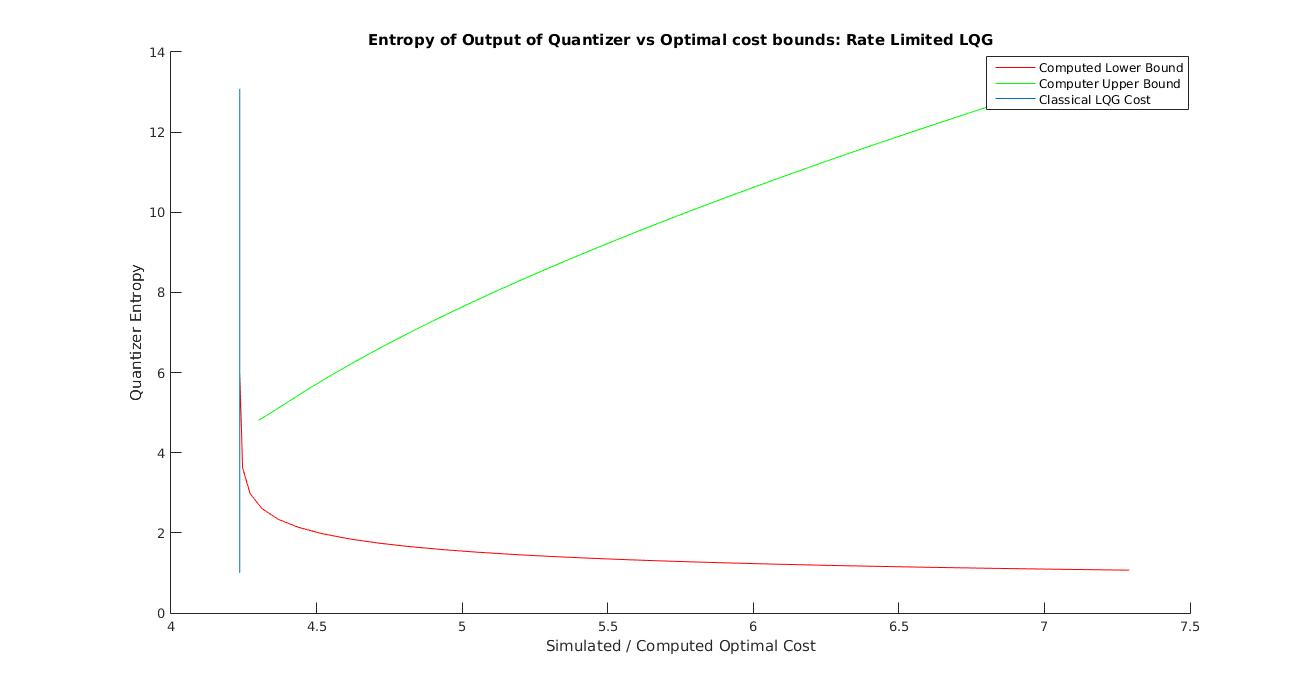
\includegraphics[scale=0.33]{lowerBound_upperBound}
			  \caption{Comparing the lower bound and upper bound to the optimal cost in the rate limited channel case. The fully observable system has the parameter $A = 2$ and the system disturbance $w$ is zero mean Laplacian with $\sigma_{w} = 1$}
			 \label{lower_upper}
		\end{figure}	
		\begin{figure}[H]
			  \centering
%			  \includesvg[width=1.0\textwidth]{block2}
%			  \def\svgscale{5.5}
			  \tiny{
%			  \input{ulft.pdf_tex}}
			\includesvg[width=16cm]{lowerBound_Simulation_Laplace_Disturbance}}
			  \caption{Comparing the lower bound to the computed optimal cost with the simulated optimal cost for system with rate limited channel. The fully observable system has the parameter $A = 2$, and the system disturbance $w$ is zero mean Laplacian with $\sigma_{w} = 1$}
			 \label{lowerboundQL_sim}
		\end{figure}	
		\begin{figure}[H]
			  \centering
%			  \includesvg[width=1.0\textwidth]{block2}
%			  \def\svgscale{5.5}
			  \tiny{
%			  \input{ulft.pdf_tex}}
			\includesvg[width=16cm]{lowerBound_Simulation_LaplaceDist_rateLimited_partiallyObservedLQG}}
			  \caption{Comparing the lower bound to the computed optimal cost with the simulated optimal cost for system with rate limited channel. The partially observable system has the parameter $A = 2$, the system disturbance $w$ is zero mean Laplacian with $\sigma_{w} = 1$ and observation noise is assumed to be zero mean Gaussian with $\sigma_{v} = 1$}
			 \label{lowerboundQL_sim_v}
		\end{figure}	
%	\begin{figure}[H]
%
%			  \centering
%%			  \includesvg[width=1.0\textwidth]{block2}
%%			  \def\svgscale{5.5}
%%			  \tiny{
%%			  \input{ulft.pdf_tex}}
%			\includegraphics[scale=0.5]{}
%			  \caption{Comparing the lower bound and upper bound to the optimal cost in the rate limited channel case. The fully observable system has the parameter $A = 2$ and the system disturbance $w$ is zero mean Laplacian with $\sigma_{w} = 1$}
%			 \label{lower_upperL}
%		\end{figure}	
		\begin{figure}[H]
			  \centering
%			  \includesvg[width=1.0\textwidth]{block2}
%			  \def\svgscale{5.5}
			  \tiny{
%			  \input{ulft.pdf_tex}}
			\includesvg[width=16cm]{loweruppersimlaplace}}
			  \caption{Comparing the lower bound and upper bound to the optimal cost in the rate limited channel case with the system simulation for simple uniform quantization scheme. The fully observable system has the parameter $A = 2$ and the system disturbance $w$ is zero mean Laplacian with $\sigma_{w} = 1$}
			 \label{lower_upper_simL}
		\end{figure}		
\chapter{Concluding Remarks}
\section{For AWGN channel}
As expected, for high SNR values, the optimal cost achieved is lower. This trait is shown by all the figures as the cost tends to the minimum value in the high SNR regime.  The important inference from the comparison between the simulations and the lower bound given in \cite{victoria} is that the lower bound is tight for non Gaussian system disturbance $w$, as shown in the figures above. The curve for simulation is close to the lower bound to minimum achievable cost and for high SNRs, the simulation matches the converse lower bound. This fact has been shown for both partially observable and fully observable cases. Hence, we can say that the lower bound given in \cite{victoria} is tight for non-Gaussian $w$.

\section{Rate Limited Channel}
Similar to previous section, it is expected that for higher entropy of the output of the quantizer (i.e. smaller quantization bins), the optimal cost would tend to the minimum. This fact is evident from the figures shown above, as we can see that the cost tends to the minimum cost ($b_{min}$) for higher values of entropy. But, the major conclusion is that even on using the simplest of schemes for quantization (a uniform quantizer), we are able to get performance cost values quite close to the lower bounds given in \cite{victoria} both for partially observable and fully observable case. However, as shown in the plots having the upper bound along with the lower bound and simulated system, the upper bound is not tight. 

\chapter{Goals}
In the coming weeks, we would be looking into the multiplicative random uncertainty in system parameter problem again. We briefly touched upon this problem in progress report I. We would like to simulate the system with random parameter under limited rate constraint to study the tightness of the lower and upper bounds which have been obtained in \cite{victoria2}. Also, we would like to extend the AWGN noise channel case to a more general vector setting where $n > 1$.

%\begin{figure}[hbt!]
%\centering
%
\includegraphics[width=.3\textwidth]{caltech.png}
%\caption{This is a figure}\label{fig:logo}
%\index{figures}
%\end{figure}


%\begin{table}[hbt!]
%\centering
%\begin{tabular}{ll}
%\hline
%Area & Count\\
%\hline
%North & 100\\
%South & 200\\
%East & 80\\
%West & 140\\
%\hline
%\end{tabular}
%\caption{This is a table}\label{tab:sample}
%\index{tables}
%\end{table}


%\endnote{Endnotes are notes that you can use to explain text in a document.}



\printbibliography[heading=bibintoc]
%
%\appendix

%\chapter{Questionnaire}
%\chapter{Consent Form}

%\printindex
%
%\theendnotes
%
%%% Pocket materials at the VERY END of thesis
%\pocketmaterial
%\extrachapter{Pocket Material: Map of Case Study Solar Systems} 
%

\end{document}
